% Präambel
\documentclass[12pt,a4paper,oneside, 
liststotoc, 					% Tabellen- und Abbildungsverzeichnis ins Inhaltsverzeichnis
bibtotoc,						% Literaturverzeichnis ins Inhaltsverzeichnis aufnehmen
titlepage, 						% Titlepage-Umgebung statt \maketitle
headsepline, 					% horizontale Linie unter Kolumnentitel
%abstracton,					% Überschrift beim Abstract einschalten, Abstract muss dazu in {abstract}-Umgebung stehen
%DIV11,							% auskommentieren, um den Seitenspiegel zu vergrößern
BCOR6mm,						% Bindekorrektur, die den Seitenspiegel um 6mm nach rechts verschiebt,
]{scrreprt}			
\usepackage{ucs} 				% Dokument in utf8-Codierung schreiben und speichern
\usepackage[utf8x]{inputenc} 	% ermöglicht die direkte Eingabe von Umlauten
\usepackage[ngerman]{babel} 	% deutsche Trennungsregeln und Übersetzung der festcodierten Überschriften
\usepackage[T1]{fontenc} 		% Ausgabe aller zeichen in einer T1-Codierung (wichtig für die Ausgabe von Umlauten!)
\usepackage{graphicx}  			% Einbinden von Grafiken erlauben
\usepackage{amsmath}
\usepackage{amsfonts}
\usepackage{amssymb}
\usepackage{mathpazo} 			% Einstellung der verwendeten Schriftarten
\usepackage{textcomp} 			% zum Einsatz von Eurozeichen u. a. Symbolen
\usepackage{listings}			% Datstellung von Quellcode mit den Umgebungen {lstlisting}, \lstinline und \lstinputlisting
\usepackage{xcolor} 			% einfache Verwendung von Farben in nahezu allen Farbmodellen
\usepackage[intoc]{nomencl}  	% zur Erstellung des Abkürzungsberzeichnisses
\usepackage{fancyhdr}			% Zusatzpaket zur Gestaltung von Fuß und Kopfzeilen
\usepackage{titleref}			% Zum referenzieren mit Überschrift
\usepackage{varwidth}			%alighn asci figure
\usepackage{chngcntr}			% Tabellen- und Abbildungsverzeichnis als fortlaufende Nummer
\usepackage{hyperref}
\usepackage[justification=centering]{caption} % Bild unterschrift mittig ausrichten
\usepackage{nameref}
\counterwithout{figure}{chapter}
\counterwithout{table}{chapter}
\usepackage{url}
\usepackage{float}
\usepackage[framemethod=tikz]{mdframed}
\usetikzlibrary{calc}
\usepackage{tikz}
\usepackage[tikz]{bclogo}
\usetikzlibrary{shapes,arrows}


% Define block styles
\tikzstyle{decision} = [diamond, draw, fill=blue!20, 
    text width=4.5em, text badly centered, node distance=3cm, inner sep=0pt]
\tikzstyle{block} = [rectangle, draw, fill=blue!20, 
    text width=5em, text centered, rounded corners, minimum height=4em, node distance=3cm]
\tikzstyle{line} = [draw, -latex']
\tikzstyle{cloud} = [draw, ellipse,fill=red!20, node distance=2cm,
    minimum height=2em]



\tikzset{
	lampsymbol/.style={%
		,scale=2,overlay}}
	
\newmdenv[nobreak,middlelinewidth=.8pt,
frametitlefont=\bfseries,
leftmargin=.3cm,rightmargin=.3cm, innerleftmargin=2cm,
skipabove=\topsep,skipbelow=\topsep,
singleextra={\path let \p1=(P), \p2=(O) in ($(\x2,0)+0.5*(2,\y1)$) node[ lampsymbol, rotate=20] {\bclampe};
	\draw[line width=.8pt,white,] ($(O|-P)+(.2cm,0)$) -- ($(P)-(.2cm,0)$); 
	\draw[line width=.8pt,white,] ($(O)+(.2cm,0)$) -- ($(P|-O)-(.2cm,0)$);
},%
]{lamp}

%\usepackage[none]{hyphenat} %deaktiviert Silbentrennung
%\usepackage{showframe}% zum Anzeigen des Seitenlayouts
%Abstand vor Chapter
\renewcommand*\chapterheadstartvskip{\vspace*{-\topskip}}
\renewcommand*\chapterheadendvskip{%
  \vspace*{1\baselineskip plus .1\baselineskip minus .167\baselineskip}}


\setlength\abovedisplayshortskip{0pt}
\setlength\belowdisplayshortskip{0pt}
\setlength\abovedisplayskip{20pt}
\setlength\belowdisplayskip{20pt}

% -----------------------------------------------------------------------------------------------------------------
% Zum Aktualisieren des Abkürzungsverzeichnisses bitte auf der Kommandozeile folgenden Befehl aufrufen :
%  makeindex Bachelorarbeit.nlo -s nomencl.ist -o Bachelorarbeit.nls
% -----------------------------------------------------------------------------------------------------------------

% Hier die persönlichen Daten eingeben:

\newcommand{\titel}{DLRG Dienstplan}
\newcommand{\untertitel}{Benutzerhandbuch für das DLRG Dienstplan-Portal
 
\url{https://dlrgdienstplan.de/}}
\newcommand{\autor}{Philippe Käufer}
\newcommand{\version}{2019.1}

\newcommand{\ovretextfalt}{%
DLRG LV Württemberg e.V. \\
Bezirk Stuttgart \\
Mühlhäuser Str. 319 \\
70378 Stuttgart \\
www.DLRG-Stuttgart.de \\
}

% Abkürzungen
\newcommand{\ua}{\mbox{u.\,a.\ }}
\newcommand{\zB}{\mbox{z.B.\ }}
\newcommand{\bs}{$\backslash$}
\newcommand{\Csharp}{C\#}

\renewcommand{\nomname}{Abkürzungsverzeichnis}
\makenomenclature 

% -------------------------------------------------------------------------------------------
% Definition der Kopf- und Fußzeilen
\lhead{}								% Kopf links
\chead{}								% Kopf mitte
\rhead{\sffamily{\titel}}				% Kopf rechts
\lfoot{}								% Fuß links
\cfoot{\sffamily{\thepage}}				% Fuß mitte
\rfoot{\sffamily{\autor}}				% Fuß rechts
\renewcommand{\headrulewidth}{0.4pt}	% Liniendicke Kopf
\renewcommand{\footrulewidth}{0.4pt}	% Liniendicke Fuß

\makenomenclature						% Abkürzungsverzeichnis erstellen

% alle Abkürzungen, die in der Bachelorarbeit verwendet werden

\nomenclature{CI}{Corporate Identity }

\nomenclature{ORM}{Objektrelationale Abbildung (object-relational mapping) }

\nomenclature{GUI}{Grafische Benutzeroberfläche oder auch grafische Benutzerschnittstelle (graphical user interface) }

\nomenclature{RWD}{(Responsive Web Design) Die Größe und Auflösung der Displays auf Laptops, Desktop-PCs, Tablets und Smartphones können erheblich variieren. Aus diesem Grund ist das Erscheinungsbild und die Bedienung einer Website stark abhängig vom Endgerät. Aufgrund dessen werden Webseiten mit einem Design ausgestattet welches sich auf die unterschiedlichen Anforderungen der Endgeräte anpassen. \cite{Responsive_Webdesign}
}

\nomenclature{Dienst}{Eine Freiwilligenarbeit in der DLRG für eine definierte Zeit. Meist im Wasserrettungsdienst oder Freibad. Der Dienst definiert wann und eventuell wie lange und wo die Freiwilligearbeit zu tätigen ist. Ein Dienst enthält eine oder mehrere zu besetzende Positionen.}

\nomenclature{Position}{Eine zu besetzende Freiwillgearbeit mit vordefinierten vorraussetzungen wie Wissen und Können (Qualifikation). Eine Position ist immer einem Dienst zugeordnet.}

\nomenclature{Qualifikation}{Ein definiertes Wissen und Können welches meist durch Besuchen von Lehrgängen und Fortbildungen in der DLRG erlangt werden kann.}				% Datei mit Abkürzungen laden


% -------------------------------------------------------------------------------------------
%                     Beginn des Dokumenteninhalts
% -------------------------------------------------------------------------------------------
\begin{document}
\setcounter{secnumdepth}{2}					% Nummerierungstiefe fürs Inhaltsverzeichnis
\setcounter{tocdepth}{2}
\sffamily									% für die Titelei serifenlose Schrift verwenden

% ------------------------------ Titelei -----------------------------------------------------

\thispagestyle{plain}
\begin{titlepage}
\enlargethispage{4.0cm}
%\sffamily 								% Serifenlose Grundschrift für die Titelseite einstellen

\begin{tikzpicture}[remember picture,overlay]%
	\node (nw) at (current page.north west) {};
	\node [xshift=0.2\paperwidth] (ne) at (nw) {};
	\node (sw) at (current page.south west) {};
	\node [xshift=0.2\paperwidth] (se) at (sw) {};

	% Farbiges Feld links
	%\filldraw[fill=yellow!90!black, draw=yellow!90!black] (nw) rectangle (se);
	\node (bard) at (nw) [anchor=north west,fill=red,minimum width=0.2\paperwidth,minimum height=\paperheight] {};

	% DLRG Wortmarke
	\node [anchor=north west,yshift=-2.5cm] at (bard.north west) {%
		
\includegraphics[width=0.185\paperwidth]{Bilder/DLRG-GELB.png}%
	};
	
	
	% Textfeld TOP
	\node (ovretext) [anchor=north west,align=left,yshift=-2.5cm,xshift=12pt,font=\sffamily] at (bard.north east) {%
		\ovretextfalt%
	};

	% Grafik mitte
	\node [anchor=north west,yshift=-2cm] at (ovretext.center) {%
		
\includegraphics[height=8cm]{Bilder/DienstplanDLRG_Kalender.png}%
	};

	% Titel
	\node (titel) [anchor=north west,yshift=-7cm+-2cm,align=left,text width=0.6\paperwidth,font=\LARGE\sffamily] 
		at (ovretext.south west) {%
		\textbf{\titel}%
	};

	% Untertitel
	\node (undertitel) [anchor=north west,yshift=-6pt,align=left,text width=0.6\paperwidth,font=\large\sffamily] 
		at (titel.south west) {%
		\untertitel%
	};

	% Author
	\node (forfattare) [anchor=south west,yshift=4cm,xshift=12pt,align=left,font=\sffamily] 
		at (bard.south east) {%
		Authoren: \autor%
	};
	
	% Logo unten rechts
	\node (logo) [anchor=south east,xshift=-18pt,yshift=18pt] at (current page.south east) {%
		
\includegraphics[width=0.2\paperwidth]{Bilder/Logo-B-Schwarz.png}%
	};
\end{tikzpicture}

\end{titlepage}
\rmfamily 				% erzeugt die Titelseite
\pagenumbering{Roman}						% große, römische Seitenzahlen für Titelei
\chapter*{Abstract} %*-Variante sorgt dafür, das Abstract nicht im Inhaltsverzeichnis auftaucht

Das DLRG Dienstplan-Portal dient zur Vereinfachung der Planung von Diensten im Ehrenamt. Der Prozess des Ausschreibens zu besetzender Dienste, der Helfer-Meldung wie auch jährlichen Statistik werden mit diesem Portal abgebildet.

\vspace*{5mm} \noindent Ziel ist es den ehrenamtlichen Helferinnen und Helfern eine Übersicht des aktuellsten Standes der Diensteinteilung wie auch selber Einflussmöglichkeiten zu geben. Die Helfer können selbst  partizipieren und Dienstwünsche direkt einreichen. 

\vspace*{5mm} \noindent Das Benutzerhandbuch für das DLRG Dienstplan-Portal hat den Zweck, eine Übersicht der Funktionen aus Sicht eines Anwenders zu geben. In diesem Dokument sind die einzelnen Funktionen und Prozesse im Detail erläutert und mit Grafiken als auch Beispielen aus der Anwendung verdeutlicht.   				% Einbinden des Abstracts

\tableofcontents							% Erzeugen des Inhalsverzeichnisses
\printnomenclature[2.0cm]					% Erzeugen des Abkürzungsverzeichnisses
\listoffigures 								% Erzeugen des Abbildungsverzeichnisses 
%\listoftables 								% Erzeugen des Tabellenverzeichnisses
\pagebreak


% --------------------------------------------------------------------------------------------
%                    Inhalt der Bachelorarbeit
%---------------------------------------------------------------------------------------------
\pagenumbering{arabic}						% arabische Seitenzahlen für den Hauptteil
\pagestyle{fancy}					
\rmfamily
\noindent

\chapter{Einführung}
\label{cha:Einleitung}


\section{Quellcode und Lizenz}
\label{sec:licens_code}
Dieses Projekt steht unter der MIT Lizenz.

\vspace*{5mm} \noindent Copyright (c) 2017 \autor

\vspace*{5mm} \noindent Hiermit wird unentgeltlich jeder Person, die eine Kopie der Software und der zugehörigen Dokumentationen (die \glqq Software \grqq) erhält, die Erlaubnis erteilt, sie uneingeschränkt zu nutzen, inklusive und ohne Ausnahme mit dem Recht, sie zu verwenden, zu kopieren, zu verändern, zusammenzufügen, zu veröffentlichen, zu verbreiten, zu unterlizenzieren und/oder zu verkaufen, und Personen, denen diese Software überlassen wird, diese Rechte zu verschaffen, unter den folgenden Bedingungen:

\noindent Der obige Urheberrechtsvermerk und dieser Erlaubnisvermerk sind in allen Kopien oder Teilkopien der Software beizulegen.

\vspace*{5mm} \noindent DIE SOFTWARE WIRD OHNE JEDE AUSDRÜCKLICHE ODER IMPLIZIERTE GARANTIE BEREITGESTELLT, EINSCHLIEßLICH DER GARANTIE ZUR BENUTZUNG FÜR DEN VORGESEHENEN ODER EINEM BESTIMMTEN ZWECK SOWIE JEGLICHER RECHTSVERLETZUNG, JEDOCH NICHT DARAUF BESCHRÄNKT. IN KEINEM FALL SIND DIE AUTOREN ODER COPYRIGHTINHABER FÜR JEGLICHEN SCHADEN ODER SONSTIGE ANSPRÜCHE HAFTBAR ZU MACHEN, OB INFOLGE DER ERFÜLLUNG EINES VERTRAGES, EINES DELIKTES ODER ANDERS IM ZUSAMMENHANG MIT DER SOFTWARE ODER SONSTIGER VERWENDUNG DER SOFTWARE ENTSTANDEN.

\chapter{Registrierung}
\label{cha:register}

Die Registrierung ist auf der Startseite links unten (Abbildung  \ref{fig:view_login} \textit{\nameref{fig:view_login}}) zu finden.

\vspace*{5mm} \noindent Alle Felder sind Pflichtangaben. Wenn die selbe E-Mail Adresse wie bei dem eigenen Facebook Account verwendet wird, ist später ein Facebook Direkt-Login möglich. Das Passwort wird in der Datenbank verschlüsselt abgelegt. Die Administratoren können das Passwort nicht einsehen.

\begin{figure}[h]
 \begin{addmargin}{-0.2\linewidth}
   \centering 
   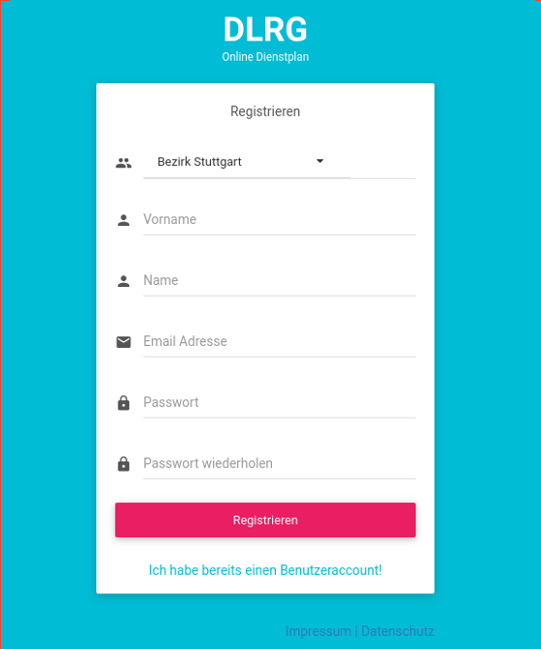
\includegraphics[width=10cm]{Bilder/view_register.png}
 \end{addmargin} 
 \caption[Registrierungs ansicht]{DLRG Dienstplan Registrierungs ansicht}
 \label{fig:view_register}
\end{figure}

\vspace*{5mm} \noindent 
Nachdem Registrungsvorgang muss der Account von einem Administrator freigeschaltet werden. Der Benutzer wird mit einer automatischen E-Mail benachrichtigt.

\noindent Nach dem erstmaligen Login sollte optional im Profil (siehe Kapitel \ref{sec:menu_profile} \textit{\nameref{sec:menu_profile}}) die Handynummer hinterlegt werden.
\chapter{Login}
\label{cha:login}

\begin{figure}[h]
 \begin{addmargin}{-0.2\linewidth}
   \centering 
   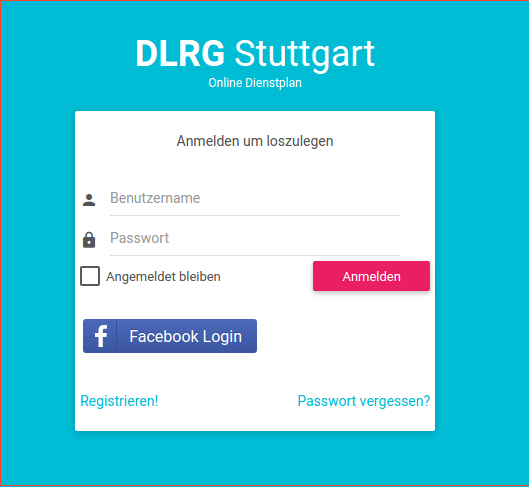
\includegraphics[width=10cm]{Bilder/view_login.png}
 \end{addmargin} 
 \caption[DLRG Dienstplan Login ansicht]{DLRG Dienstplan Login ansicht}
 \label{fig:view_login}
\end{figure}
\chapter{Menü}
\label{cha:menu}
\chapter{Qualifikationen}
\label{cha:qualification}
Ein Benutzer bekommt durch das Zuweisen von Qualifikationen die Rechte im Dienstplan eingetragen zu werden. Bei Zuweisung einer Qualifikation wir der Benutzer mit einer E-Mail benachrichtigt. Die Aktuell zugewiesenen Qualifikationen können über den Schnellzugriff (\ref{sec:menu_qualification} \textit{\nameref{sec:menu_qualification}}) eingesehen werden.

\noindent Qualifikationen sind ein zentraler Bestandteil um die Berechtigungen für Positionen zu erlangen. Positionen welche eine entsprechende Qualifikation voraussetzt, kann nur durch Benutzer mit dieser Qualifikation besetzt werden.

\noindent Bei neu erlangen von Qualifikationen (z.B. durch erfolgreichen Abschluss von Lehrgängen) müssen diese durch die Administratoren zugewiesen werden. Der Benutzer muss hier mit den Administratoren in Kontakt treten.

\vspace*{5mm} \noindent Sollte ein Benutzer zugriff auf mehrere Gliederungen haben, müssen die Qualifikationen von jeder Gliederung einzeln zugeteilt werden.
\chapter{Dashboard}
\label{cha:dashboard}

Das Dashboard bietet Überblicke und Statistiken:

\begin{itemize}
\item Geleistete Dienste: Summe der Dienste bei welchem der Benutzer eine Position übernommen hatte.
\item Total Geleistete Dienste: Summe der Positionen welche von allen geleistet wurde.
\item Noch nicht besetzte Dienste: Summe der zukünftig noch nicht besetzten Positionen. Hier werden nur Positionen welche für eine Mindestbesatzung relevant sind aufgezählt.
\item Hall of Fame: Benutzer mit den am meisten geleisteten Diensten. 
\end{itemize}

\noindent Darunter sind News (Kapitel \ref{cha:nachrichten}) wie auch neue Infos zu finden. Diese werden meist ebenfalls per E-Mail den Benutzern zugestellt.

\begin{figure}[h]
 \begin{addmargin}{-0.2\linewidth}
   \centering 
   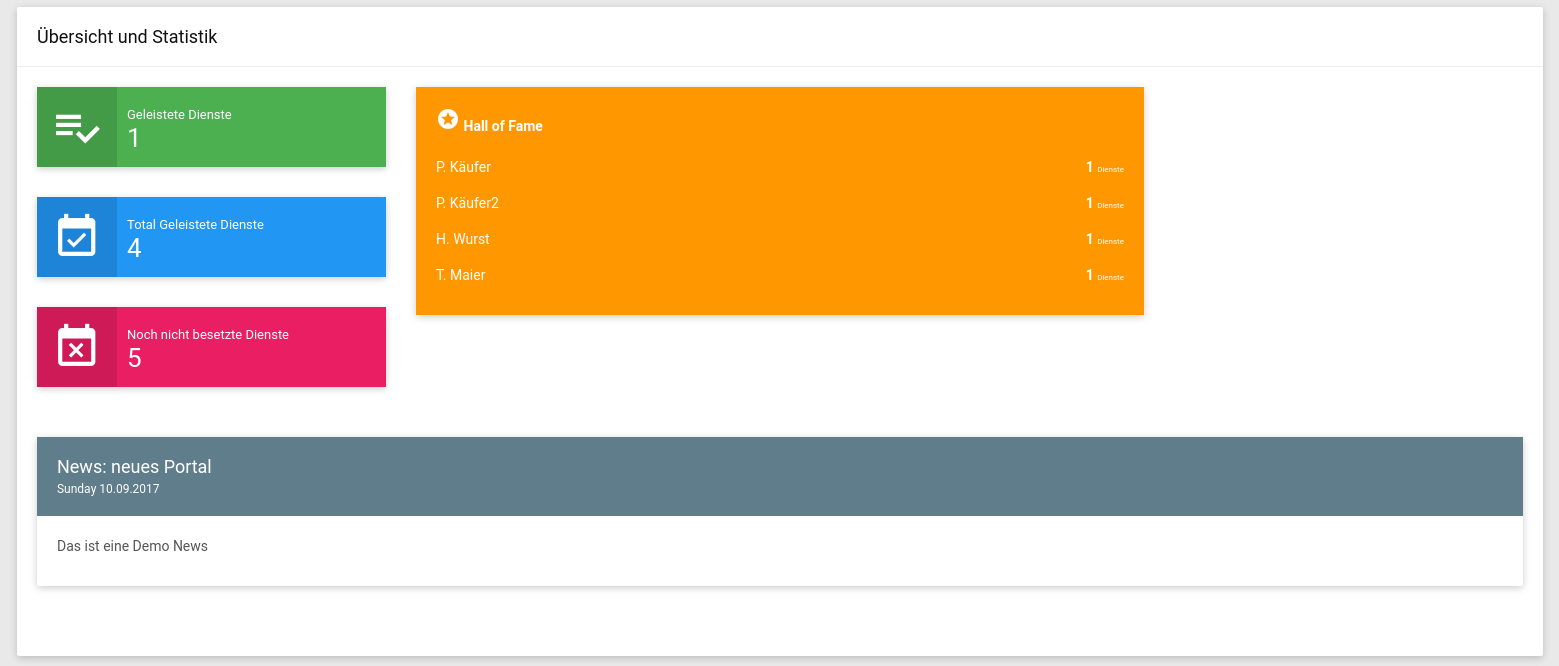
\includegraphics[width=20cm]{Bilder/view_overview.png}
 \end{addmargin} 
 \caption[Dashboard ansicht]{DLRG Dienstplan Dashboard ansicht}
 \label{fig:view_overview}
\end{figure}
\chapter{Dienste}
\label{cha:dienste}
Die Dienstübersicht zeigt alle zukünftigen Dienste absteigend sortiert nach Datum. Jeder Dienst wird als Block klar getrennt und übersichtlich dargestellt. In Abbildung \ref{fig:view_service} \textit{\nameref{fig:view_service}} ist ein einzelner Dienst exemplarisch abgebildet.

\begin{figure}[h]
 \begin{addmargin}{-0.2\linewidth}
   \centering 
   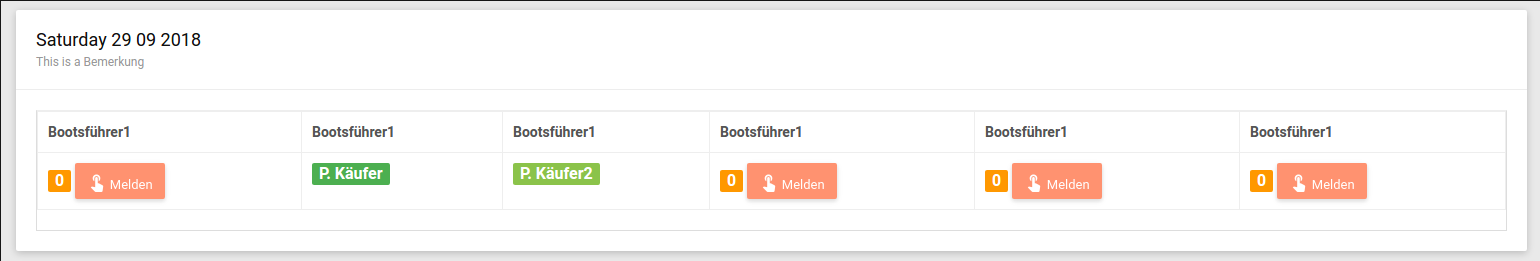
\includegraphics[width=20cm]{Bilder/view_service.png}
 \end{addmargin} 
 \caption[Dienste Übersicht]{DLRG Dienstplan Dienste Übersicht}
 \label{fig:view_service}
\end{figure}

\noindent Jeder Dienst ist mit Tag und Datum beschriftet. Darunter kann eine Bemerkung bzw. Beschreibung hinterlegt sein. Die einzelnen Positionen des Dienstes werden als Tabelle dargestellt.
\noindent Dem Benutzer kann eine Position in fünf verschiedenen Ansichten präsentiert werden mit welchen er zum teil Interagieren kann.
Diese sind in der folgenden Tabelle aufgezeigt. Beispiele beziehen sich immer auf die Abbildung \ref{fig:view_service} \textit{\nameref{fig:view_service}}

\begin{itemize}
\item Melden (bsp. Position 4): Diese Position ist noch nicht zugeteilt. Der Benutzer kann sich hierzu melden.
\item Melden deaktiviert (bsp. Position 1): Diese Position ist noch nicht zugeteilt. Der Benutzer hat aber nicht die entsprechende Qualifikation und kann sich somit für die Position nicht melden.
\item Position bestätigt (bsp. Position 2): Die Position ist bereits zugeteilt.
\item Position bestätigt (bsp. Position 3): Diese Position ist an den Benutzer zugeordnet. Alle zugeordneten Positionen des eigenen Benutzers werden zur besseren Übersicht hellgrün dargestellt.
\item Für Position gemeldet, noch nicht bestätigt (bsp. Position 5): Für diese Position hat der Benutzer sich bereits gemeldet. Solange dies durch die Administratoren noch nicht bestätigt ist, kann die Meldung zurück gezogen werden.
\end{itemize}

\noindent Die Zahl in den Orangenen Kästen vor dem Melde Button (bsp Position 4) gibt an, wie viele andere Benutzer sich bereits für diese Position gemeldet haben. Ein Benutzer kann sich für beliebig viele Positionen eines Dienstes melden. Ebenso können beliebig viele Benutzer sich für eine Position melden. Durch die Administratoren wird nur einer Benutzer für eine Position bestätigt.

\noindent Positionen können Kommentare beinhalten (bsp. Position 1). Mit Kommentaren können geteilte Positionen (Position 1 nur bis 14 Uhr) realisiert werden. Des weiteren können mit Kommentaren auch auf Besonderheiten zu dieser Position hingewiesen werden.


\section{Mobile Ansicht}
\label{sec:dienste_mobile}
Die GUI auf Mobilgeräten, wie \zB Smartphones oder Tablets, weicht von der Desktopversion leicht ab. Die einzelnen Dienste sind eingeklappt und können mit einem Tippen auf den kleinen Pfeil oder das Datum ausgeklappt werden (\ref{fig:view_service_mobile_close} \textit{\nameref{fig:view_service_mobile_close}}). 


\begin{figure}[h]
 \begin{addmargin}{-0.2\linewidth}
   \centering 
   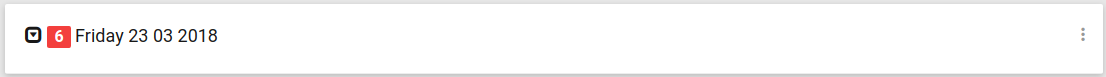
\includegraphics[width=20cm]{Bilder/view_service_mobile_close.png}
 \end{addmargin} 
 \caption[Dienste Übersicht Mobil]{DLRG Dienstplan Dienste Übersicht Mobil eingeklappt}
 \label{fig:view_service_mobile_close}
\end{figure}


\noindent Die rot hinterlegte Zahl zwischen dem kleinen Pfeil und dem Datum gibt die Anzahl der noch nicht zugewiesenen Positionen eines Dienstes an. In Abbildung \ref{fig:view_service_mobile} \textit{\nameref{fig:view_service_mobile}} ist die Zahl 6 dort zu sehen da wie in der ausgeklappten Ansicht zu sehen ist, 6 Positionen noch nicht zugewiesen wurden.

\begin{figure}[h]
 \begin{addmargin}{-0.2\linewidth}
   \centering 
   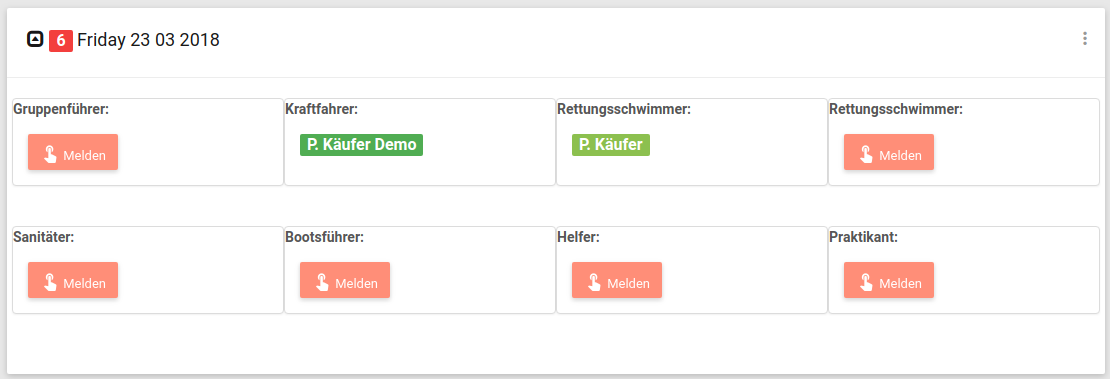
\includegraphics[width=20cm]{Bilder/view_service_mobile.png}
 \end{addmargin} 
 \caption[Dienste Übersicht Mobil Ausgeklappt]{DLRG Dienstplan Dienste Übersicht Mobil ausgeklappt}
 \label{fig:view_service_mobile}
\end{figure}
\chapter{Nachrichten}
\label{cha:nachrichten}
\chapter{Prozesse}
\label{cha:prozesse}
In diesem Kapitel werden ausgewählte Standartprozesse zur Übersicht und späteren Orientierung der Benutzer definiert.

\section{Benutzer registrieren}
\label{sec:process_register}
Jeder Helfer benötigt einen eigenen Benutzeraccount. Dieser kann auf der Startseite unter \glqq Registrieren\grqq ~angelegt werden. Der Benutzer muss zunächst durch einen Administrator der Gliederung freigeschaltet werden. Der Benutzer wird via E-Mail über die Freischaltung informiert. Nach dem ein Benutzer Freigeschaltet wurde, wird der Administrator die entsprechenden Qualifikationen zuweisen. Wenn nicht alle bzw. die entsprechenden Qualifikationen zugewiesen wurden, sollten die Administratoren der Gliederung darauf aufmerksam gemacht werden.

\noindent \textit{Es ist zu empfehlen die selbe E-Mail Adresse wie bei Facebook zu verwenden. Hierdurch kann später das \glqq oneclick\grqq ~Login verfahren verwendet werden.}

\section{Dienst melden}
\label{sec:process_position_apply}
Für das Melden zu einem Dienst muss lediglich der entsprechende Tag gesucht werden. Bei Positionen mit entsprechender Voraussetzung an Qualifikationen kann der Benutzer sich direkt melden.

\noindent \textit{Ein Benutzer sollte sich bei einem Dienst zu mehreren Positionen melden. Die Administratoren werden nur einen bestätigen und haben somit mehr Flexibilität beim Besetzen der Dienste.}

\section{Dienst Aufteilen}
\label{sec:process_service_split}
Es ist möglich einzelne Dienste bzw. dessen Positionen in zwei Schichten aufzuteilen. Bereits geteilte Dienste sind an einem Kommentar der Position zu erkennen. Ist ein Dienst der geleistet werden will nicht aufteilt, werden die Administratoren durch einem freundlichen Hinweis per E-Mail dies einrichten.

\section{Dienst Absagen}
\label{sec:process_service_cancel}
Sollte ein Benutzer einen bereits gemeldeten Dienst absagen müssen, kann er dies, wenn noch nicht bestätigt, über \glqq Meldung zurückziehen\grqq ~(siehe Kapitel \ref{cha:dienste} \nameref{cha:dienste}) selber durchführen. Ist der Dienst bereits bestätigt, muss mit den Administratoren Kontakt aufgenommen werden.

\section{Für weitere Gliederung registrieren}
\label{sec:process_apply_client}
Benutzer können oben über das Schnellzugriff-Menü (\ref{sec:menu_applyclient} \nameref{sec:menu_applyclient}) eine Zuordnung zu weiteren Gliederungen beantragen. Der Benutzer muss durch einen Administrator der entsprechenden Gliederung freigeschaltet werden. Mit einer E-Mail wird der Benutzer über die Freischaltung informiert. Nach der Freischaltung, wird der Administrator die entsprechenden Qualifikationen zuweisen. Wenn nicht alle bzw. die entsprechenden Qualifikationen zugewiesen wurden, sollten die Administratoren der Gliederung darauf aufmerksam gemacht werden.
\chapter{Administrator}
\label{cha:administrator}
In diesem Kapitel wird die Sicht eines Administrators beleuchtet und dessen spezielle Berechtigungen und Aufgaben dargelegt.

\vspace*{5mm} \noindent Die Rolle des Administrators wird in Verbindung zu Gliederungen gesetzt. Ein Benutzer kann also Administrator von einer oder mehreren Gliederungen sein. Eine Gliederung muss durch mindestens einen, kann aber durch mehrere Benutzer administriert werden.

\vspace*{5mm} \noindent Die Navigation ist zusätzlich zu den Funktionen eines Benutzers um folgende Einträge erweitert: 
\begin{itemize}
	\item Benutzer (Kapitel: \ref{sec:admin_benutzerverwaltung})
	\item Dienste bestätigen
	\item Dienst anlegen (Kapitel: \ref{sec:admin_service})
	\item Nachricht erstellen (Kapitel: \ref{sec:admin_news})
	\item Qualifikationen (Kapitel: \ref{sec:admin_qualifikationsverwaltung})
	\item Client (Kapitel: \ref{sec:admin_gliederungsverwaltung})
\end{itemize}

\section{Gliederungsverwaltung}
\label{sec:admin_gliederungsverwaltung}
Über den für Administratoren eingeblendeten Menüpunkt \noindent (Abbildung \ref{fig:view_client} \textit{\nameref{fig:view_client}}, Markierung \textit{1}, rechts oben) kann die Eigenschaften-Seite einer Gliederung aufgerufen werden um diese zu konfigurieren.

\begin{itemize}
	\item[\textbf{Name:}] Name der Gliederung. Dieser wird oben links, in der Gliederungsauswahl wie auch bei der Registrierung verwendet.
	\item[\textbf{Start der Saison:}] Gibt den Saison-Start an. Statistiken und Graphen welche nur für eine Saison Daten aggregieren, werden zu dem Datum zurückgesetzt.
	\item[\textbf{Dienstbeginn:}] Angabe wann ein Dienst standardmäßig beginnt. Dies dient einer schnelleren Administration und wirkt sich als vorausgefüllte Formularfelder aus.
	\item[\textbf{Dienstende:}] Angabe wann ein Dienst standardmäßig endet. Dies dient einer schnelleren Administration und wirkt sich als vorausgefüllte Formularfelder aus.
	\item[\textbf{Automatismen:}]
	\begin{itemize}
		\item Wöchentliches versenden des Wachplans: Wenn dies ausgewählt ist, wird jeden Montag der Wachplan unter folgenden Bedingungen versendet: Es existiert in den Kommenden zwei Wochen mindestens ein Dienst. 
		
		\noindent Die Mail wird den Wachplan für die nächsten zwei Monate beinhalten.
	\end{itemize}
	\item[\textbf{Mailingliste:}]
	\begin{itemize}
		\item Checkbox: Wenn dies ausgewählt ist, werden E-Mails nicht an jeden Nutzer einzeln sondern an eine Mailingliste versendet. Hierdurch können auch Personen außerhalb des Dienstplan-Portals Informationen wie z.B. Nachrichten oder den wöchentlichen Dienstplan erhalten.
		\item Mailingliste E-Mail: Definiert an welche E-Mail Adresse (Mailingliste) gesendet werden soll, wenn die Checkbox gesetzt ist.
	\end{itemize}
	\item[\textbf{Absender:}]
	\begin{itemize}
		\item Absender Name: Name welcher als Absender von ausgehenden Mails angezeigt wird.
		\item Antworten an E-Mail Adresse: E-Mail Adresse von welcher E-Mails versendet werden. Hier sollte eine ...@gliederung.dlrg.de Adresse hinterlegt sein.
	\end{itemize}
\end{itemize}

\begin{figure}[h]
	\begin{addmargin}{-0.2\linewidth}
		\centering 
		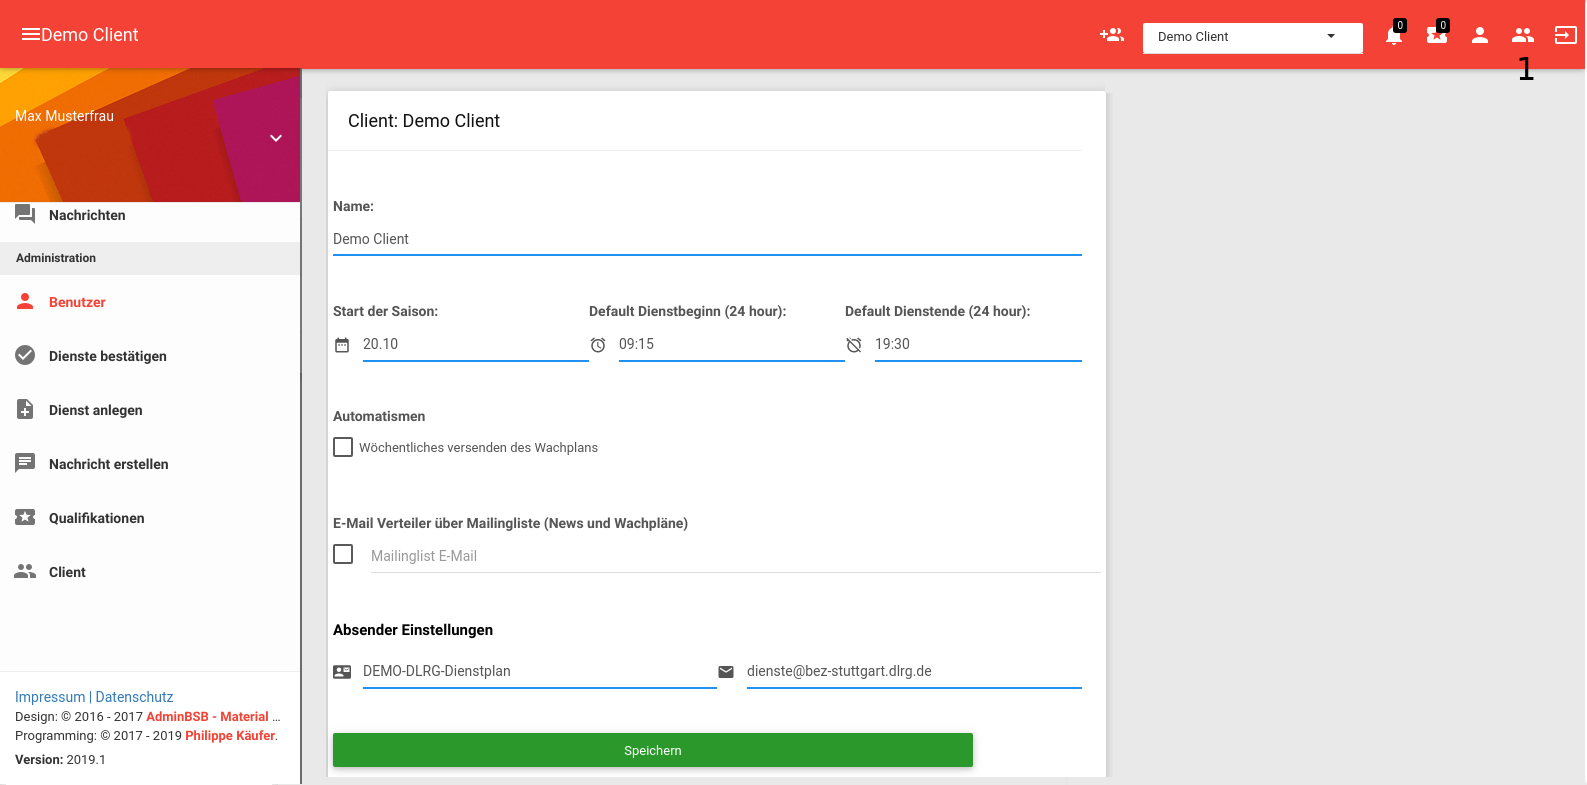
\includegraphics[width=20cm]{Bilder/view_admin.png}
	\end{addmargin} 
	\caption[Gliederungsverwaltung]{DLRG Dienstplan Gliederungsverwaltung}
	\label{fig:view_client}
\end{figure}

\section{Benutzerverwaltung}
\label{sec:admin_benutzerverwaltung}
In dem Menüpunkt Benutzer werden alle Benutzer der aktuellen Gliederung tabellarisch aufgelistet. Über diese Tabelle stehen drei Aktionen zu Verfügung:

\begin{table}[H]
	\centering
	\begin{tabular}{ll}
		
\includegraphics[width=1.5cm]{Bilder/edit.png} & Editieren der Eigenschaften eines Benutzers. \\[10pt]
		
\includegraphics[width=1.5cm]{Bilder/approve.png}	& Benutzer für die Gliederung freigeben. \\[10pt]
		
\includegraphics[width=1.5cm]{Bilder/remove.png} & Die Zuordnung des Benutzer mit der aktuellen Gliederung löschen. \\
	\end{tabular}
	%\caption{Übersicht Icons und Funktionen Benutzerverwaltung}
	%\label{fig:admin_benutzerverwaltung}
\end{table}

\section{Qualifikationsverwaltung}
\label{sec:admin_qualifikationsverwaltung}
Qualifikationen stellen die zentrale Komponente um Benutzen die Berechtigung zu erteilen, Positionen zu besetzen. Hierfür werden zunächst Qualifikationen angelegt. Darauf aufbauend sind beim anlegen eines Dienstes den einzelnen Positionen basierend auf Qualifikationen zuzuordnen. Im Dienstplan können folgend nur Benutzer, welche diese Qualifikation zugewiesen bekommen haben, sich bei entsprechenden Positionen melden. Beispiel: Zunächst wird eine Qualifikation Sanitäter angelegt. Diese Qualifikation wird Benutzern über die \ref{sec:admin_benutzerverwaltung} \nameref{sec:admin_benutzerverwaltung} zugewiesen. Werden Dienste mit Positionen \glqq Sanitäter\grqq{} angelegt, können nur entsprechende Nutzer mit der Qualifikation \glqq Sanitäter\grqq{} sich für diese Position melden.

\vspace*{5mm} \noindent Das anlegen von Qualifikationen bedingt folgende Eingaben:

\begin{itemize}
	\item[\textbf{Name:}] Name der Qualifikation.
	\item[\textbf{Abkürzung:}] Abkürzung der Qualifikation. Diese Abkürzung wird verwendet, wenn der Name für Eingabefelder, Anzeigen oder Ausdrucke zu lang ist. Es wird empfohlen hier max. 5 Zeichen zu verwenden.
	\item[\textbf{Default:}] \glqq Soll die Qualifikation bei anlegen von einem Service automatisch erstellt werden?\grqq{} Ist die Checkbox markiert, werden beim erzeugen eines Dienstes automatisch Positionen mit dieser Qualifikation angelegt.
	\item[\textbf{Default Anzahl:}] Gibt die Anzahl der Positionen an, welche beim erzeugen von Diensten automatisch angelegt werden.
	\item[\textbf{Erforderlich:}] Ist eine Position bei Diensten zwingend erforderlich, kann diese markiert werden (ref.: \ref{sec:admin_service} \nameref{sec:admin_qualifikationsverwaltung}). Diese Checkbox gibt den Standartwert vor, wenn eine Position mit dieser Qualifikation automatisch oder manuell einem Dienst hinzugefügt wird.
\end{itemize}

\begin{lamp}[frametitle={Qualifikationen Benutzern zuweisen}]
	Über die Benutzerverwaltung können Qualifikationen den Benutzern zugewiesen werden. Die Zuweisung erfolgt getrennt für jede Gliederung/Mandant. Mit dem Zuweisen werden Benutzer automatisch via E-Mail über diese Aktion informiert.
\end{lamp}

\section{Dienstverwaltung}
\label{sec:admin_service}
Dienste bestehen aus mindestens einer und beliebig vielen Positionen. Über den Menüpunkt Dienste (Kapitel \ref{cha:dienste} \nameref{cha:dienste}) werden alle angelegten Dienste der aktuellen Saison angezeigt. Das Anlegen von Diensten unterliegt den Administratoren einer Gliederung und erfolgt unter dem Menüpunkt \glqq Dienst anlegen \grqq{}. Ein Dienst hat folgende Eigenschaften:

\begin{itemize}
	\item[\textbf{Datum:}] Datum des Dienstes.
	\item[\textbf{Freigabe:}] Wenn Personen sich auf eine Position melden, müssen diese erst von einem Administrator bestätigt werden.
	\item[\textbf{Bemerkung:}] Dieses Feld kann z.B. für dem Namen einer Veranstaltung o.ä. verwendet werden. Alternativ ist dieses leer zu lassen.
	\item[\textbf{Positionen:}] Es können beliebig viele Positionen mit folgenden Eigenschaften hinzugefügt werden:
	\begin{itemize}
		\item \textbf{Qualifikation:} Definiert die Qualifikation für diese Position.
		\item \textbf{Person:} Zugewiesene Person. Beim anlegen kann dies auf \glqq -- Bitte wählen -- \grqq{} gesetzt bleiben. Soll Direkt eine Person zugewiesen werden ist diese aus dem Dropdown zu wählen. Die Liste ist nach Nachnamen sortiert, auch wenn die Anzeige den ersten Buchstabe des Vornamens mit anzeigt. Personen mit passender Qualifikation sind grün hinterlegt. Personen welche Positionen neu zugeteilt wurden, werden via E-Mail automatisch darüber in Kenntnis gesetzt.
		\item \textbf{Kommentar:} Optinales Feld für z.B. Infos wenn eine Position eine extra Sonderaufgabe zugewiesen wird oder eine andere Dienstzeit aufweist.
		\item \textbf{Erforderlich:} Ist diese Position zwingend zu besetzten oder optional? Hat Auswirkung auf die Rote Zahl der freien Dienste in der Dienstauflistung (\ref{cha:dienste} \nameref{cha:dienste}) sowie auf die Statistiken.
	\end{itemize}
\end{itemize}
Melden sich Personen selbständig für Dienste bzw. deren Positionen, werden alle Admins via E-Mail darüber in Kenntnis gesetzt. Die Freigabe erfolgt über die Admins auf der Dienste Ansicht (ref.: \ref{cha:dienste} \nameref{cha:dienste}). Eine Freigabe löst wiederum eine automatische Benachrichtigung der betroffenen Person aus.

\section{Nachrichtenverwaltung}
\label{sec:admin_news}
Verfasste Nachrichten werden an alle Nutzer versendet. Je nach Einstellung der Gliederung wird eine E-Mail an die Mailingliste oder aber an jeden Benutzer einzeln versendet.
Nachrichten werden unter dem Menüpunkt \glqq Nachrichten\grqq{} Chronologisch aufgelistet. Zusätzlich wird die neueste Nachricht auf dem Dashboard (ref.:\ref{cha:dashboard} \nameref{cha:dashboard}) dargestellt.
\chapter{Aussicht}
\label{cha:aussicht}
Das DLRG Dienstplan-Portal soll stetig weiterentwickelt und verbessert werden. Hierzu sind im allgemeinen Feedback und Vorschläge immer willkommen!

\vspace*{5mm} \noindent Fehler, Erweiterungen und Wünsche werden bei der Codeverwaltung mit geführt: \url{https://github.com/Philhil/DienstplanDLRG/issues}
Direkte Einflussnahme und Diskussion zu Verbesserungen kann dort geschehen oder über E-Mail.

\vspace*{5mm} \noindent Funktionen die in Zukunft folgen:

\begin{itemize}
\item Mobile Ansicht: Die Mobile Ansicht für Smartphones soll optimiert werden.
\item Spezial Aufgaben: Es ist wünschenswert Spezialaufgaben wie z.B. Kochen für einen Dienst im DLRG Dienstplan-Portal festzulegen. 
\item Message Funktion innerhalb eines Dienstes: Für die vorab Kommunikation einer Dienst-Mannschaft ist es hilfreich dort eine direkte Kontaktmöglichkeit zu schaffen. Denkbar: Gruppenführer kann E-Mail versenden, Whatsapp Gruppe erstellen...
\item Kalender Funktion: Jeder Benutzer kann für sein Handy/Desktop Kalender den Dienstplan abbonieren. Bestätigte (und gemeldete?) Dienste würden so direkt im gewohnten Kalender vermerkt.
\item Hier könnte deine Idee stehen!
\end{itemize}


% ---------------------------- Literaturverzeichnis ----------------------------------------------

\begin{thebibliography}{999999}

%\bibitem {Buchtitel} Author: \emph{Buchtitel}, Erscheinungsort: Verlag, Jahr

\bibitem {Responsive_Webdesign} Wikipedia: \emph{Responsive Webdesign}, \url{https://de.wikipedia.org/wiki/Responsive_Webdesign}, 15 12 2017.

\bibitem {Facebook_Login} Facebook: \emph{Facebook Login für das Web mit dem JavaScript-SDK}, \url{https://developers.facebook.com/docs/facebook-login/web}, 28 12 2017.


\end{thebibliography}

% ------------------------------- Anhang ---------------------------------------------------------

\begin{appendix}
\clearpage
\pagenumbering{Roman}						% römische Seitenzahlen für Anhang
\end{appendix}


\end{document}